% The first argument is the \documentclass, which tells latex which template
% we're using to build this document. It's usually safe to just use "article".
\documentclass{article}

% include some packages...
\usepackage{fullpage} % change settings for a smaller margin
\usepackage{graphicx} % gives access to the \includegraphics commands
\usepackage{amsfonts}
\usepackage{float}
\usepackage{enumitem}
\usepackage{caption}
\usepackage[export]{adjustbox}
\usepackage{bookmark}
\graphicspath{{./images/}}

% tell Latex to use no paragraph indentation, but leave some space between
% paragraphs
\setlength{\parindent}{0in}
\setlength{\parskip}{0.1in}

\newcommand{\tib}[1]{\textit{\textbf{#1}}}
\newcommand{\code}[1]{\texttt{#1}}

% these commands merely set the values for the title/date/author; they don't put
% them in the document... see \maketitle below
\title{CS Department Automated Information Timeline \\ Assignment 6.3: GRASP Concepts}
\date{\today}
\author{Matthew Hays, Pawan Bhandari, Sarah Faron, Tim Klimpel}

% all document content goes between \begin{document} and \end{document}
\begin{document}

% this command actually creates the title/date/author in the document
\maketitle
\newpage
\tableofcontents
\listoffigures
\newpage
\section{Introduction}
\subsection{Purpose}
The purpose of this assignment is to work as a team and collaboratively to identify General Responsibility Assignment Software Patterns (GRASP) in the design of the CS Department Automated Information Timeline project. The team met multiple times over the course of a few days to work together and identify the GRASP concepts. Section 2 of this document consists of the identified GRASP concepts and section 3 contains the annotated sequence diagrams.

\section{GRASP concepts}
Table below lists all classes that appear in the sequence diagrams and under GRASP concept the class is suited for.
\begin{table}[H]
    \centering
    \begin{tabular}{| c | c | c | c |}
    \hline
        \textbf{Controller} & \textbf{Creator} & \textbf{Information Expert} & \textbf{Low Coupling/High Cohesion}\\
        \hline
         EventController & EventMapper & EventRepository & EventService \\
         ReviewController & EventRepository & NotificationRepository & NotificationService \\
         PostController & NotificationRepository & PostRepository & ReviewService \\
         MediaController & NotificationMapper & MediaRepository & PostService \\
           & PostRepository & PageRepository & MediaService \\
           & MediaRepository &  & DisplayService \\
           & PageRepository &  & PageService \\
           &  &  & \\
    \hline
    \end{tabular}
    \caption{Classes with the identified GRASP concepts}
    \label{tab:my_label}
\end{table}
Low coupling and high cohesion is achieved by clearly separating out Controller, Service and Repository actions so that each class is only responsible for its specific layer of the application.  This is also a core part of the MVC pattern which is known to be loosely coupled and highly cohesive.\\
The mapper classes (EventMapper and NotificationMapper) were also identified as a creators because they are meant to be injected in service classes to create objects to be used as entities. Mapper classes support low coupling by removing a need for mapping user inputs directly to domain object needs and high cohesion by dealing only with JSON Serialization/deserialization of Event/EventDTO objects.

\section{Annotated Sequence diagrams}
A subset of sequence diagrams are annotated with the identified GRASP concepts and these are included below. These sequence diagrams cover all the classed and the GRASP patterns they implement.

\subsection{Create Event}
        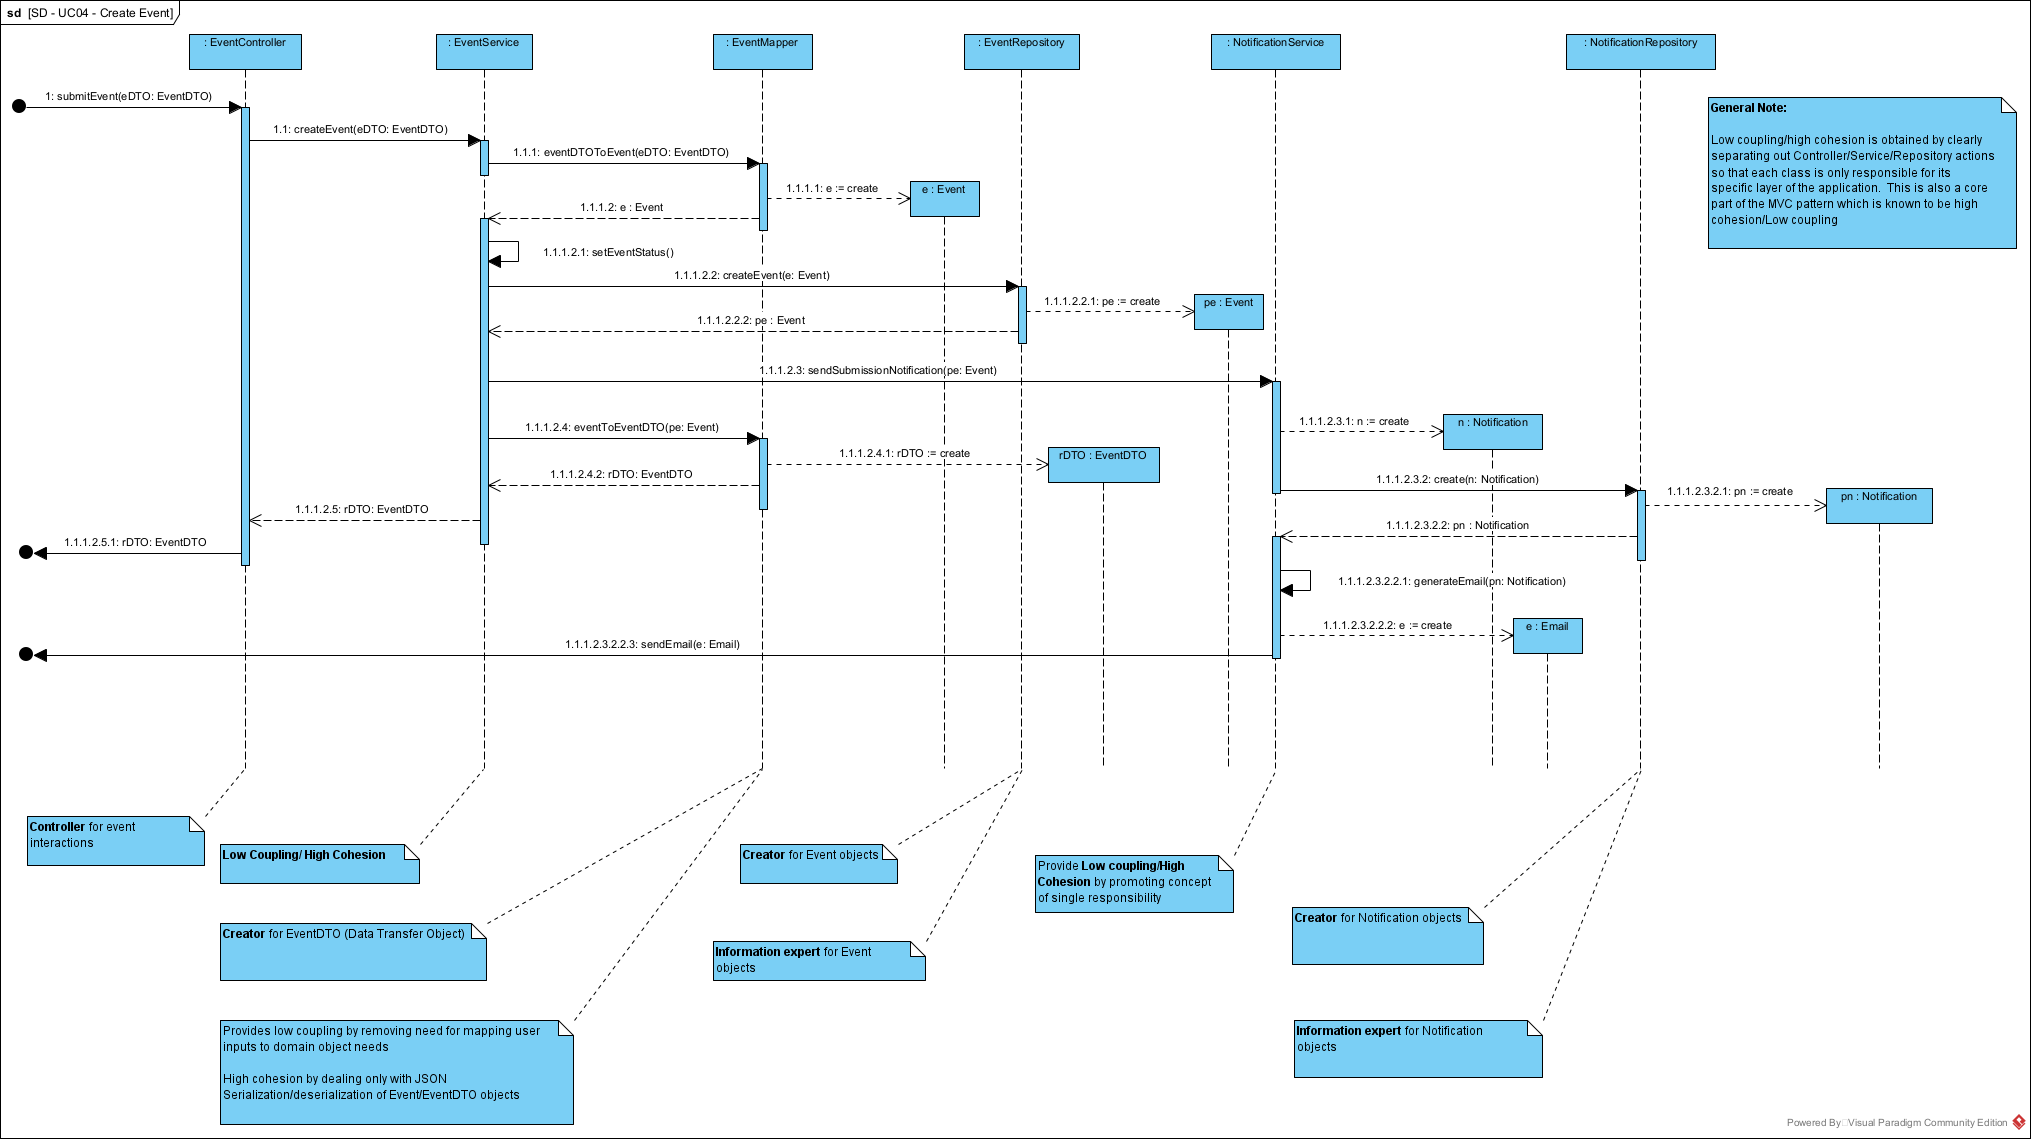
\includegraphics[scale=0.34]{images/SD-UC04-CreateEvent.png}
        \captionof{figure}{Sequence Diagram: Create Event}
        \label{fig:SD-CreateEvent}
\subsection{Review for Approval}
        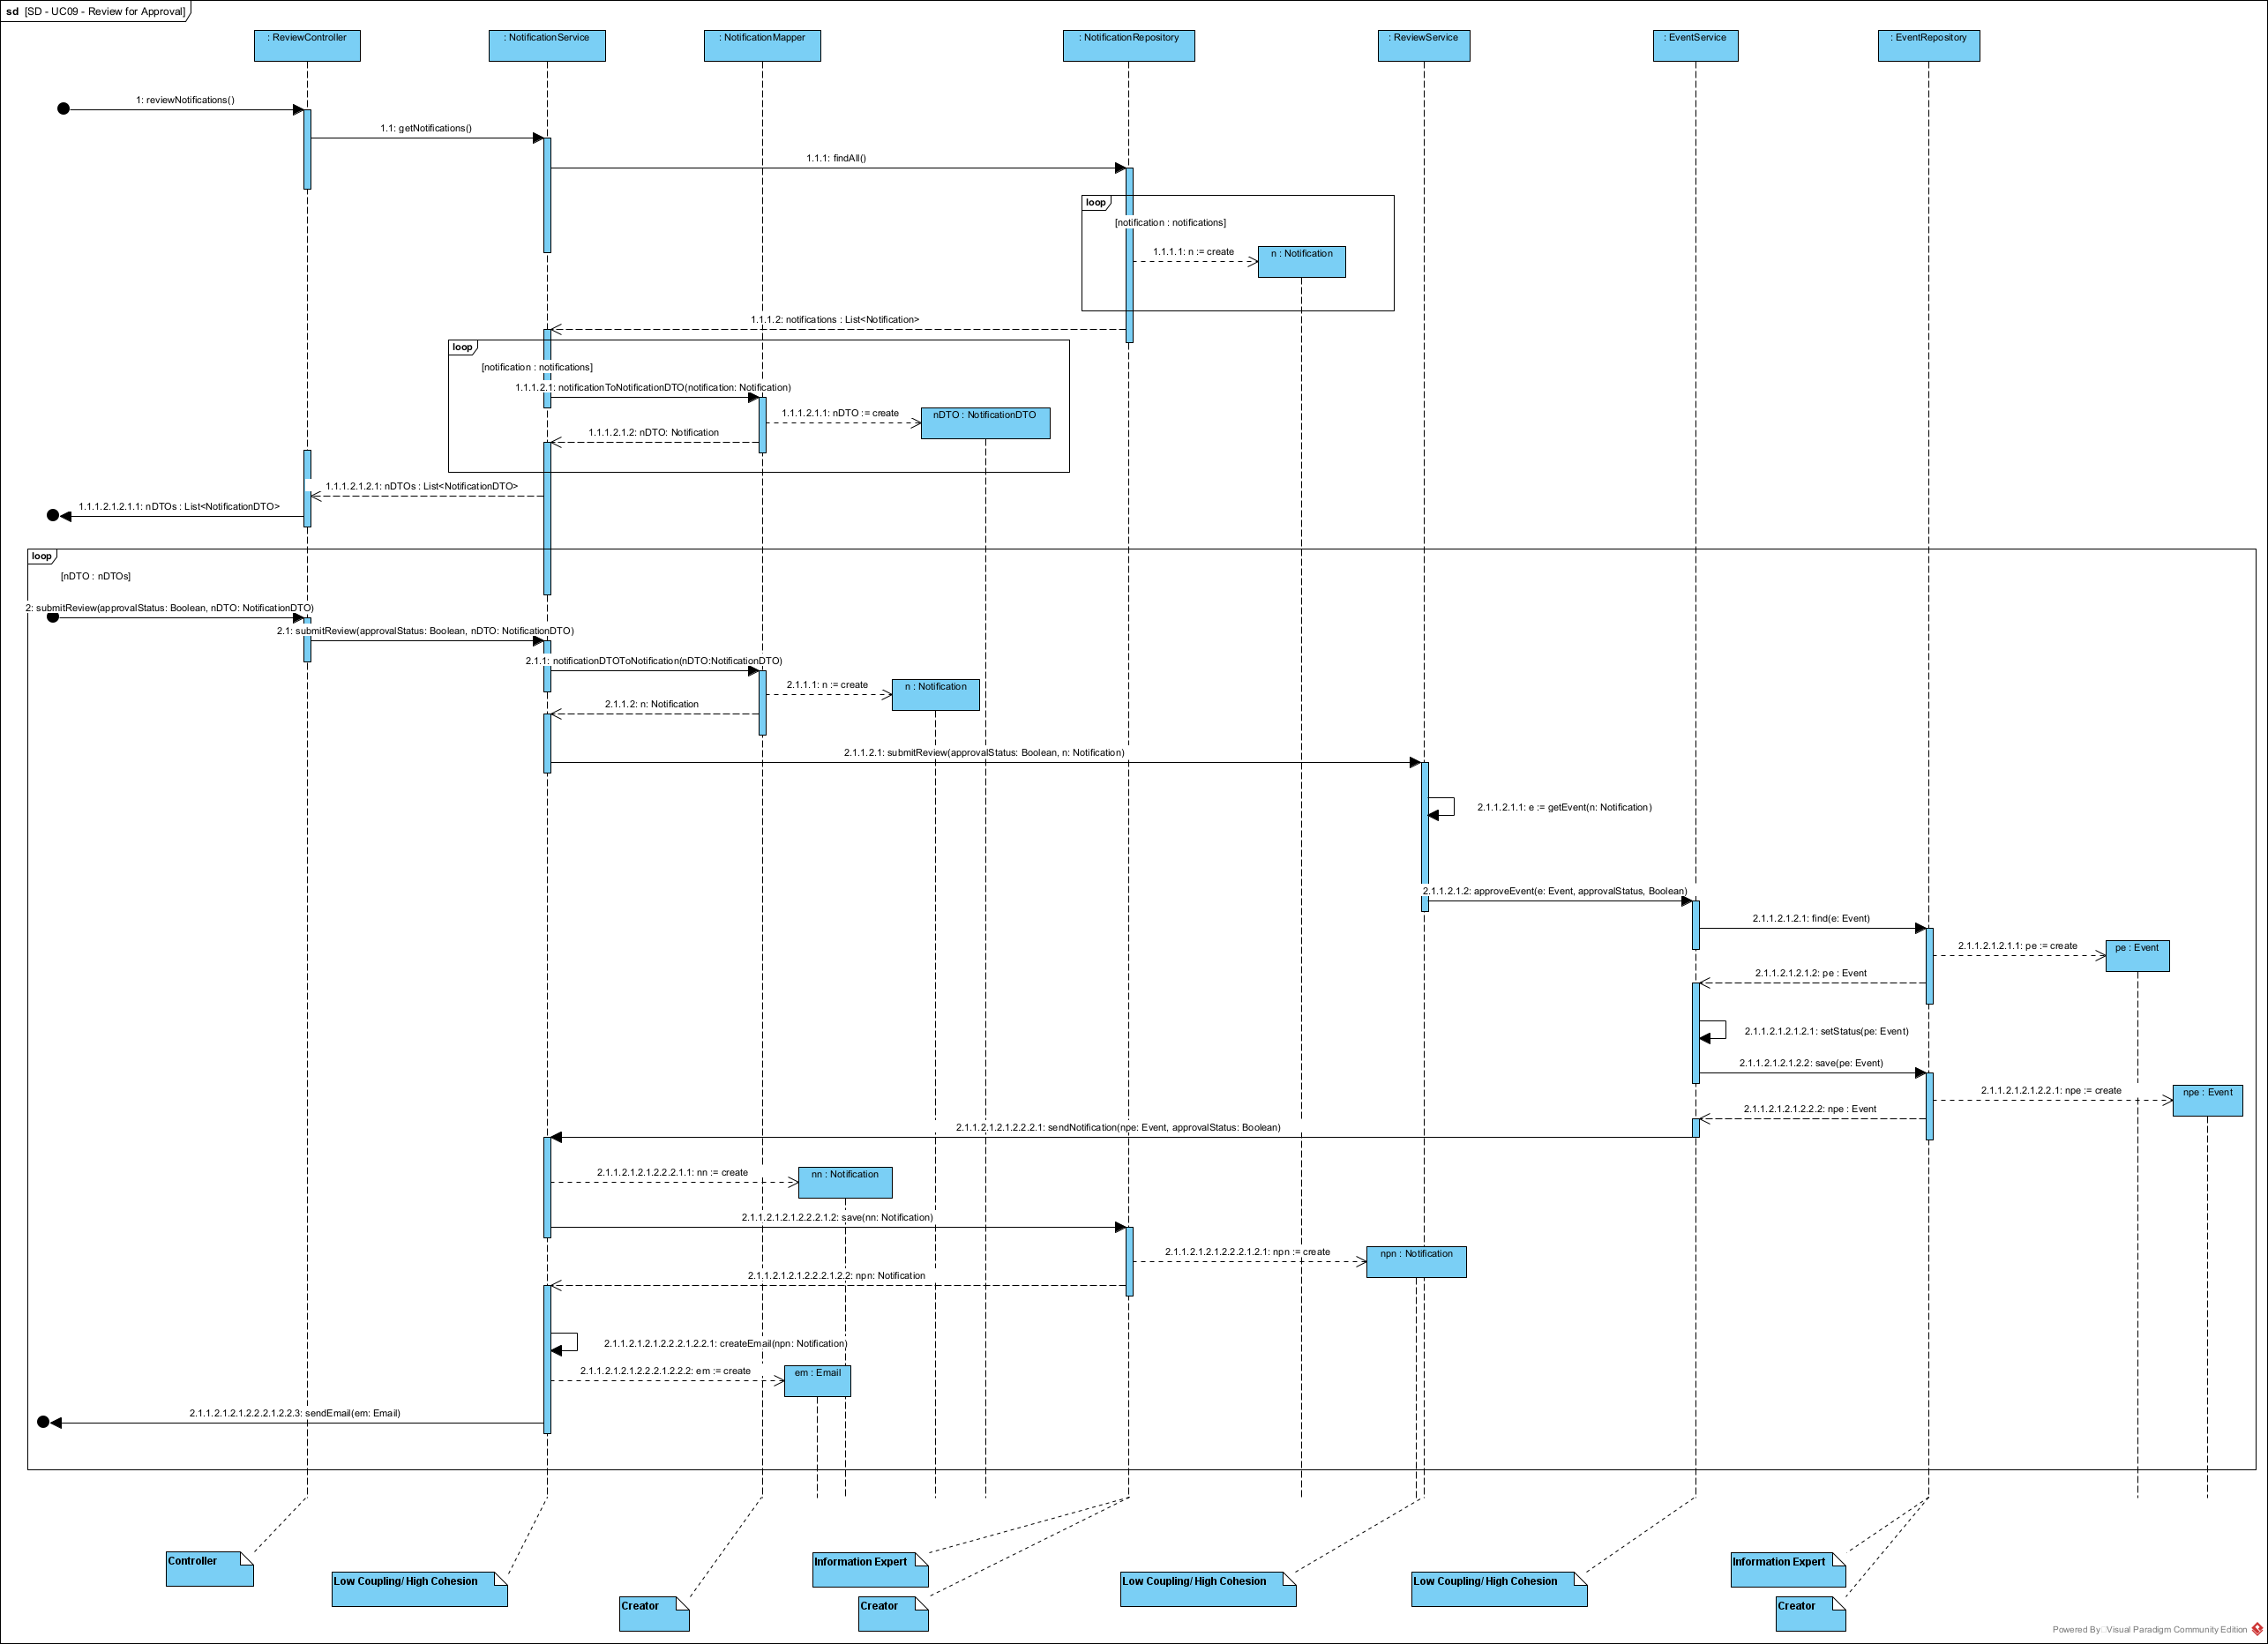
\includegraphics[scale=0.27]{images/SD-UC09-ReviewForApproval.png}
        \captionof{figure}{Sequence Diagram: Review for Approval}
        \label{fig:SD-ReviewForApproval}
\subsection{Edit Post}
        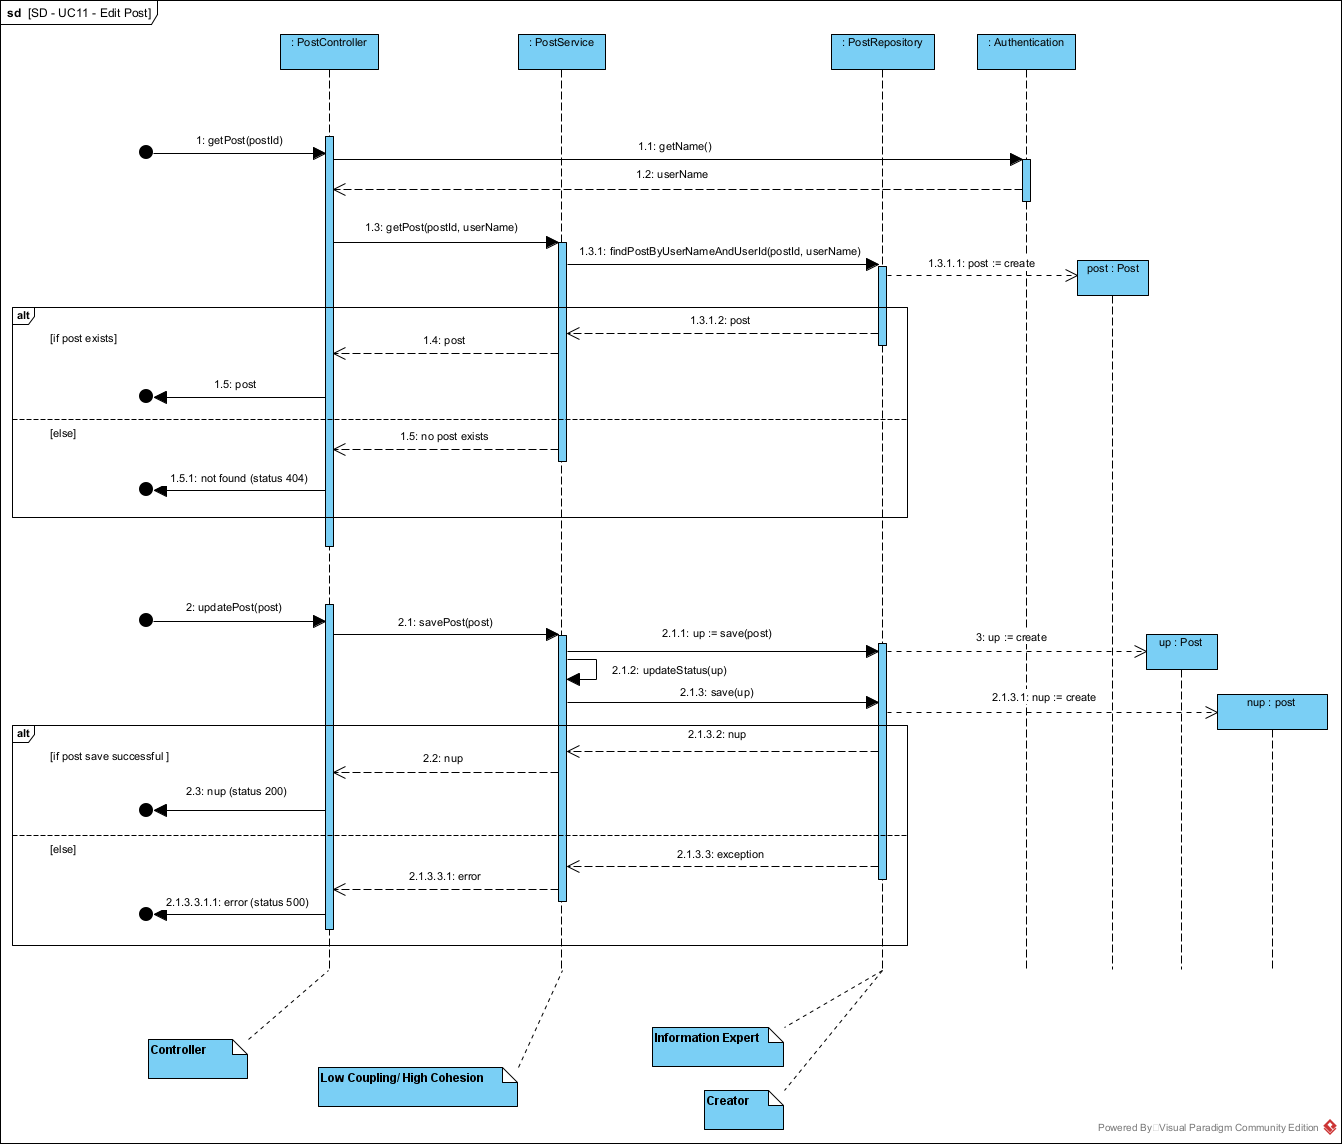
\includegraphics[scale=0.5]{images/SD-UC11-EditPost.png}
        \captionof{figure}{Sequence Diagram: Edit Post}
        \label{fig:SD-EditPost}
\subsection{Manage Displayed Media}
        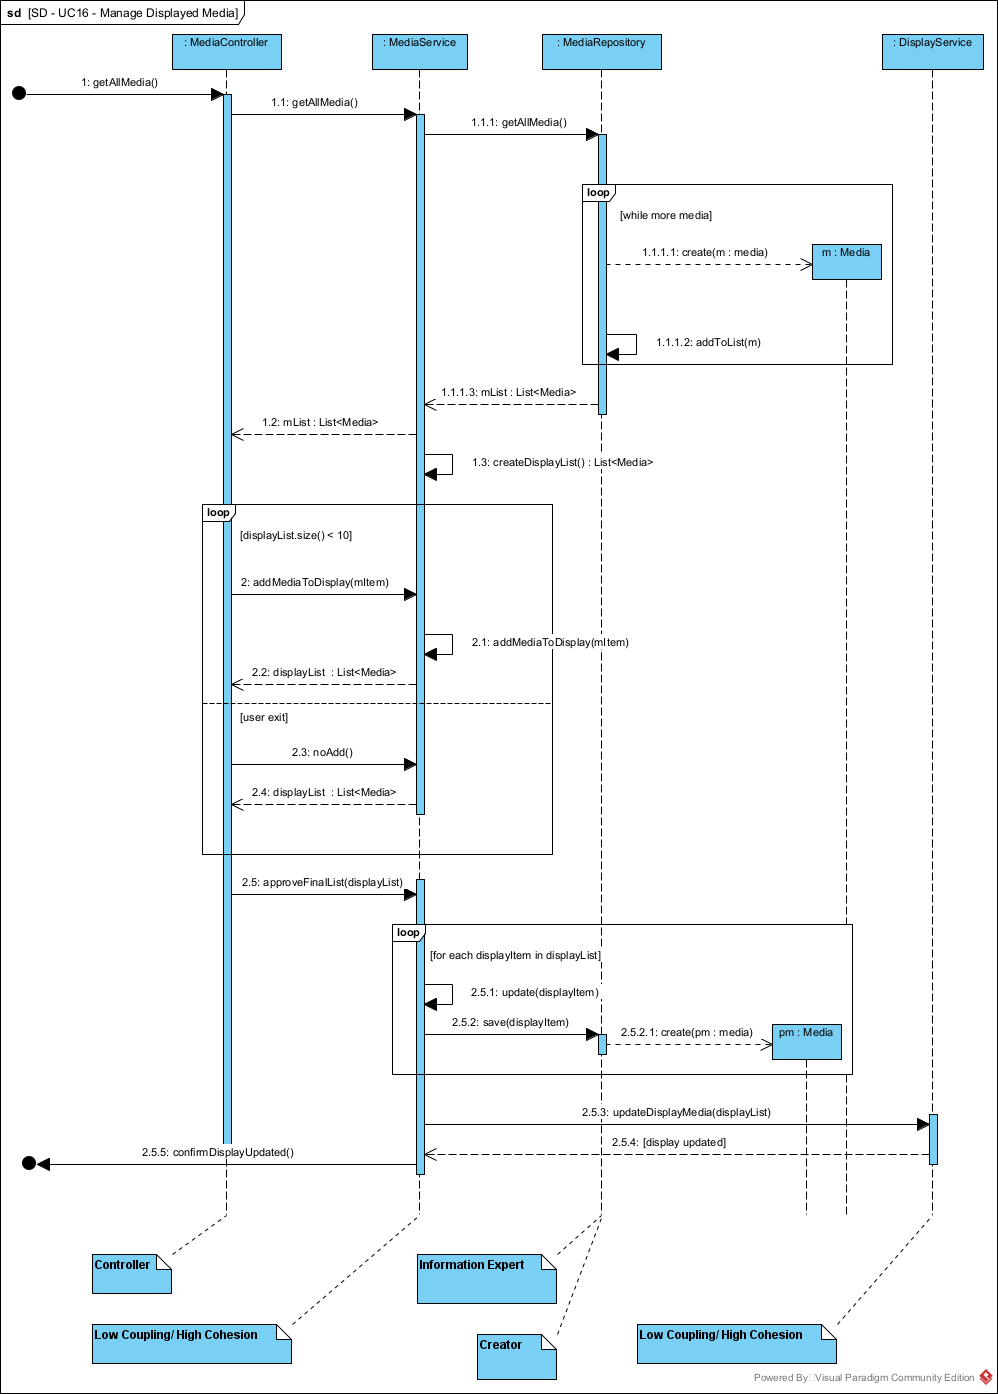
\includegraphics[scale=0.55]{images/SD-UC16-ManageDisplayedMedia.png}
        \captionof{figure}{Sequence Diagram: Manage Displayed Media}
        \label{fig:SD-ManageDisplayedMedia}
\subsection{Add Page to Event}
        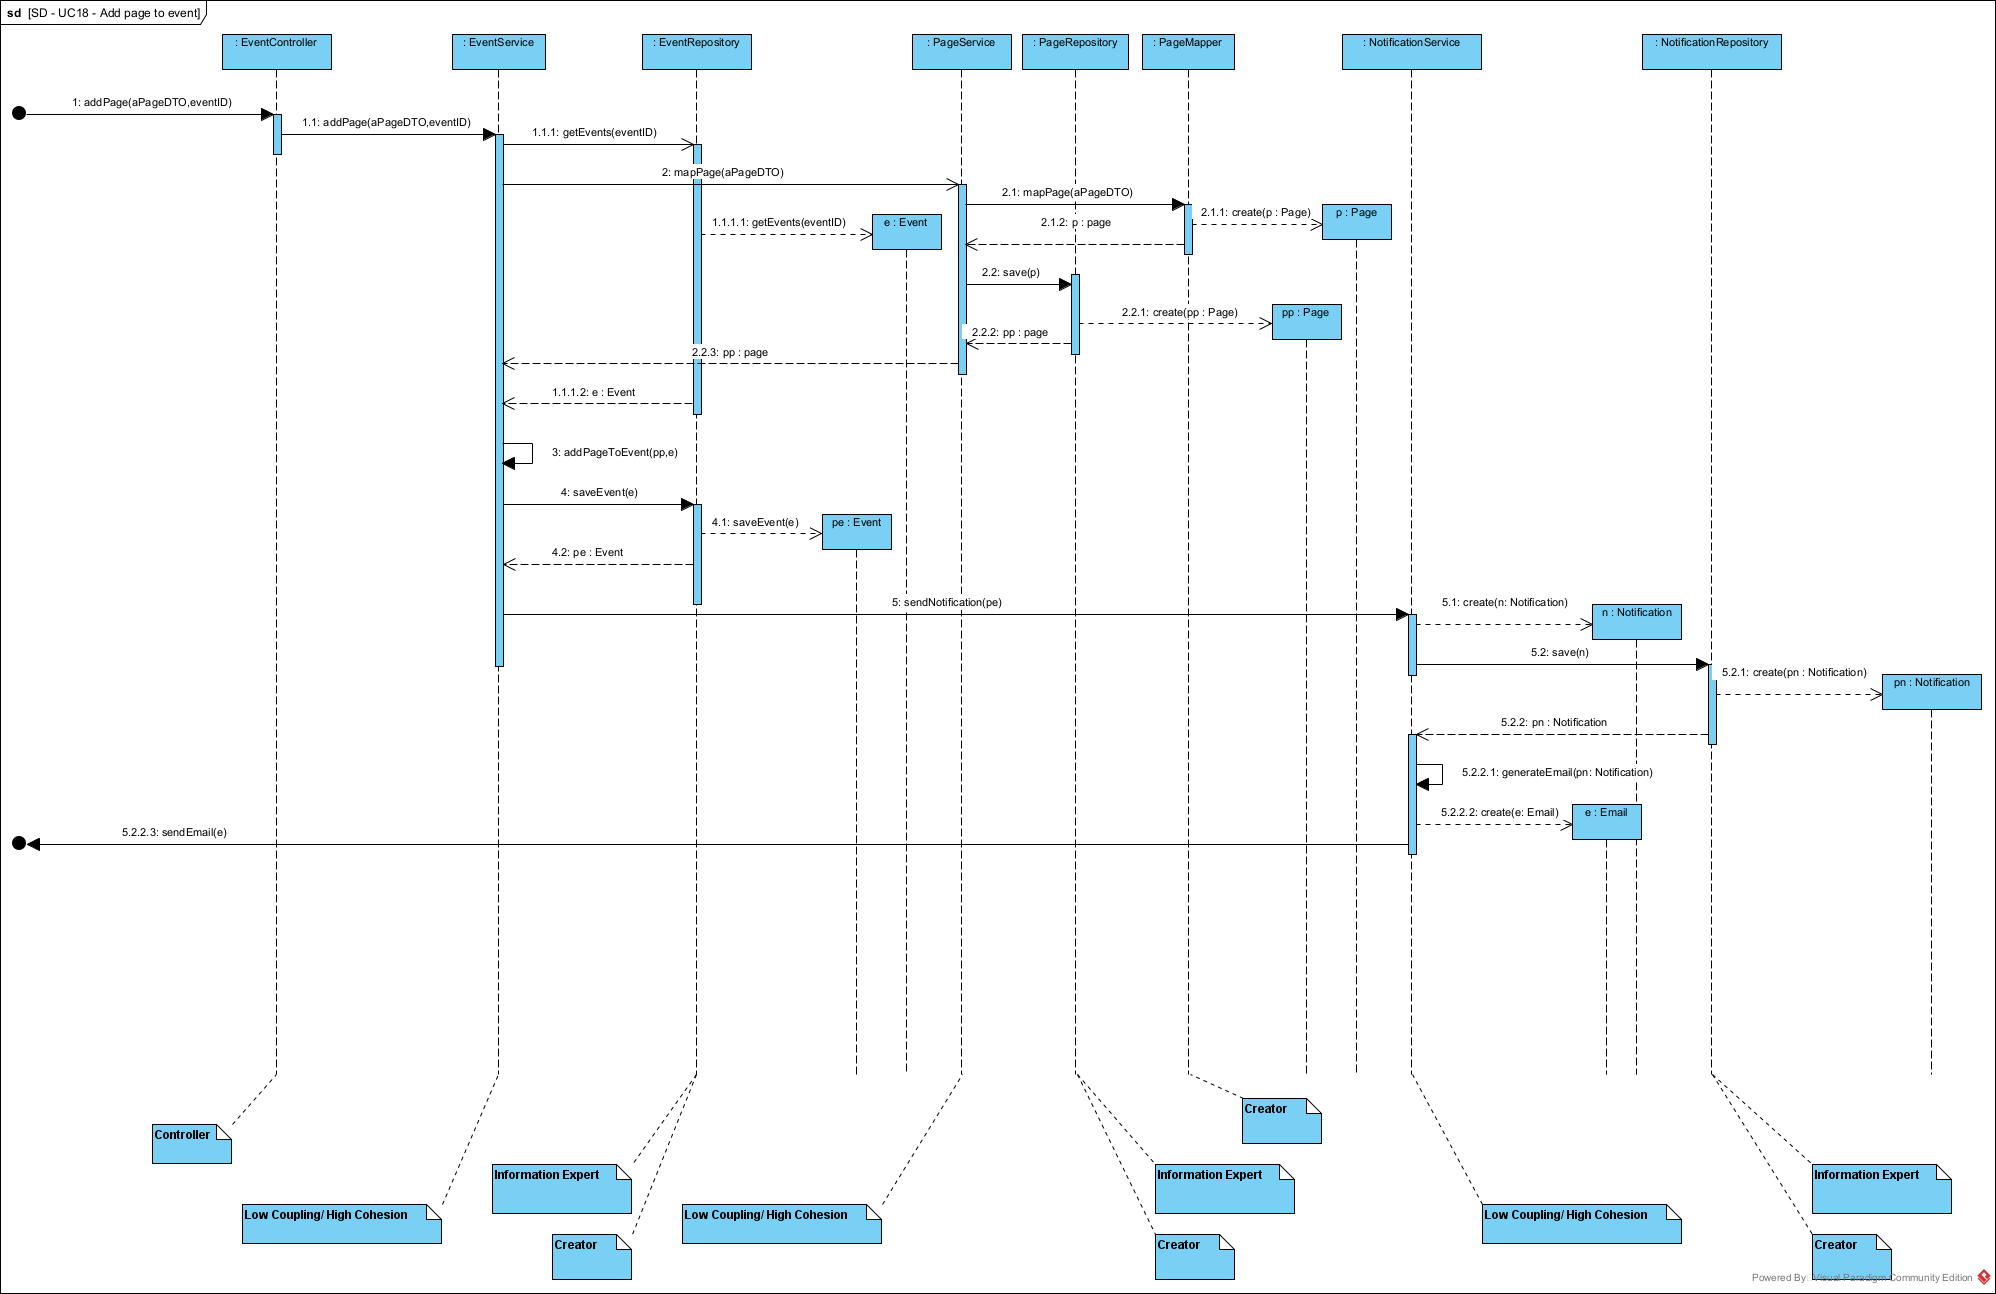
\includegraphics[scale=0.35]{images/SD-UC18-AddPageToEvent.png}
        \captionof{figure}{Sequence Diagram: Add page to Event}
        \label{fig:SD-AddPageToEvent}

\end{document}